
Google Docs made real-time editing in browsers easy for millions of
users. However, Google mediates real-time editing sessions with central servers
raising issues on privacy, censorship, and economic intelligence. It also raises
scalability issues in terms of the number of participants.  Despite that small
groups currently constitute the main range of users, events such as massive
online lectures, TV shows, conferences gather larger groups.  Google Docs
supports large groups but only the first fifty users can edit, next users have
their rights limited to document reading.  We think that real-time editors
should allow editing at anytime and anywhere, whatever the number of
participants.

%% In this paper we focus on building a real-time editor that supports privacy
%% and that adapts \TODO{gently} from small groups to large groups

Decentralized real-time editors~\cite{oster2006data, sun1998operational,
  sun2009contextbased} do not require intermediate servers and by the same
settle privacy issues. However, scalability issues remain.  Addressing
scalability requires finding a good trade-off between communication, space and
time complexities. Achieving a sublinear communication complexity compared to
the number of participants is crucial for supporting large groups.

%% But consistency maintenance of documents requires each message to piggyback
%% additional information which greatly impacts the communication complexity.

To provide availability and responsiveness of documents, real-time editors use
optimistic replication~\cite{saito2005optimistic} of sequences, text documents
being sequences of characters. As such, each user manages a local copy of the
document and directly performs her modifications on it. Changes are broadcast to
all replica owners where they are integrated. The system is correct iff the
replicas integrating an identical set of operations converge to an equivalent
state, i.e., users read a same document~\cite{shapiro2011conflict}.

Decentralized algorithms of Operational
Transformation~\cite{sun2009contextbased} (OT) require piggybacking a state or a
context vector in order to detect concurrent operations. Unfortunately, state
vectors grow linearly with respect to the number of members that ever
participated in the authoring. Hence, these approaches are efficient for small
groups of users, but poorly scale to highly dynamic large groups of users and
high network latency.

Conflict-Free Replicated Data Types~\cite{shapiro2011comprehensive} (CRDTs) do
not pay the price of concurrency detection by providing commutative
operations. However, they require to piggyback unique and immutable identifiers
on every operation broadcast on the network. The size of this identifier is the
key for the communication complexity and consequently the scalability of the
approach. Two classes of CRDTs designed for sequences exist:
\begin{itemize}
\item CRDTs such as WOOT~\cite{oster2006data} piggyback a constant-size
  identifier which is optimal. However, it requires to keep tombstones, i.e., it
  marks elements as removed and hide them from the users. An empty document may
  store thousands of deleted elements. Tombstones degrade integration time of
  operations. This integration time blocks the user and eventually make the
  real-time editor unusable. Removing tombstones requires garbage
  collecting algorithms that do not scale.
\item CRDTs such as Logoot~\cite{weiss2010logootundo} do not require tombstones
  but piggyback variable size identifiers. Depending on the identifier
  allocation strategy, the size of identifiers may grow linearly with the
  document size, increasing the communication cost. Balancing the structure
  requires consensus algorithms that do not scale.

  In previous works, we proposed an identifier allocation strategy called
  \LSEQ~\cite{nedelec2013concurrency, nedelec2013lseq}. It aims to avoid such
  balancing mechanism by sublinearly upper-bounding the space complexity of its
  identifiers. It is conjectured to have a polylogarithmic growth of the
  identifiers size $\mathcal{O}((\log d)^2)$ where $d$ is the document
  size.
  
  Figure~\ref{fig:complexity} shows the results of experiments where variable
  size identifier approaches~\cite{nedelec2013lseq, preguica2009commutative,
    weiss2009logoot} were asked to generate identifiers at the end of the
  document (top figure), and at random position in the document (bottom
  figure). The documents reach half a million characters. We observe that while
  random editing leads to logarithmic growth of identifiers in any of the
  approaches, an editing behavior as trivial as left-to-right editing
  constitutes an issue. Treedoc and Logoot expose linear growth. \LSEQ provides
  sublinearly upper-bounded identifiers. As such, \LSEQ outperforms
  state-of-the-art approaches and scales in terms of document size.
\end{itemize}

The contributions of this paper are threefold:
\begin{itemize}
\item Compared to previous work~\cite{nedelec2013concurrency, nedelec2013lseq},
  we prove the upper bounds on space and time complexities of \LSEQ. This result
  opens the way for building decentralized and scalable real-time editors.
\item We describe all the outlines to develop a distributed
  collaborative editor for massive editing of large documents.
\item We built a real-time decentralized editor running in web
  browsers\footnote{\url{https://github.com/Chat-Wane/CRATE}}. In the Grid'5000
  testbed, we launched an editing session involving up till 600 connected
  browsers. The resulting documents reach millions of characters. It validates
  the scalability of the editor built on top of \LSEQ.
\end{itemize}

\begin{figure}
  \centering
  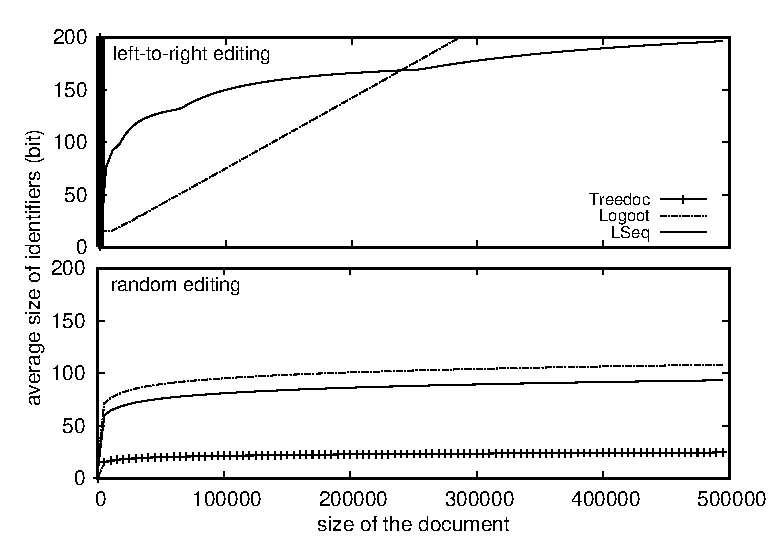
\includegraphics[width=0.8\textwidth]{img/complexity.eps}
  \caption{\label{fig:complexity} Average size of identifiers generated by CRDTs
    for sequences using variable size identifiers. The top figure concerns
    repeated insertions at the end of the document. The bottom figure concerns
    insertions at random positions in the document.}
\end{figure}

%%% Local Variables: 
%%% mode: latex
%%% TeX-master: "../paper"
%%% End: 
